% 2. Fragen zur Vorbereitung

\chapter{Theoretischer Hintergrund}
\label{chap:fvz}

\section{Arten und Vergleich der Mikroskope}
\label{sec:artenEM}

\subsection*{Raster-Elektronenmikroskop (REM)}
Bei einem REM wird durch einen Elektronenstrahl die zu untersuchende Probe zeilenförmig abgerastert. Dabei wird die Topografie (Oberfläche), die Kristallstruktur un Materialunterschiede der Probe auf einen Bildschirm mittels Sekundärelektronen (SE, inelastische Stöße) und Rückstoßelektronen (RE, elastische Stöße) mit entsprechenden Detektoren abgebildet. Weiterhin lässt ein REM eine Röntgenanalyse zu, wodurch auch eine Elementanalyse der Probe möglich ist. \citep{RasterEM}
\begin{itemize}
    \item Auflösung: $\sim$ \SI{10}{\nano\metre}\\
    Das Auflösungvermögen ist dabei von dem Strahlendurchmesser und dem Abbildungsignal abhängig und beträgt zwischen \SI{1}{\nano\metre} $\sim$ \SI{2}{\nano\metre} in günstigen Verhältnissen. \citep{WikiREM}
    \item Eindringtiefe: $\sim$ \SI{1}{\micro\metre}
    \item Probe: Vakuumstabil und trocken mit leitender Oberflächenschicht 
\end{itemize}
Das REM und seine Funktionsweise wird in weiteren Kapitel noch genauer betrachtet.

\subsection*{Transmission-Elektronenmikroskop (TEM)}
Bei einem TEM werden dünne Probe wird mit Elektronen durchstrahlt, welche durch die Streuung ihre Bewegungsrichtung ändern und ihre Energie durch inelastische Stöße verlieren. Die Elektronen, welche das Material durch elastische Stöße unter Erhaltung des Eintrittswinkels verlassen, werden in der hinteren Brennebene fokussiert. Die gestreuten Elektronen werden mit einer Blende abgeschirmt. Entweder wird dann das \textit{Zwischenbild} (vergrößertes Lichtbild) oder das \textit{Elektronenbeugungsbild} (Fokusebene) betrachtet. 
\begin{itemize}
    \item Auflösung: einige \si{\nano\metre} bis \si{\micro\metre}\\
    Dabei hängt die Auflösung von der Beschleuigungsspannung (80 $\sim$ 400\si{\kilo\volt}) und der Materialdicke ab. 
    \item Probe: Ultradünne Schnitte notwendig (10–\SI{100}{\nano\metre}) \citep{WikiTEM}
\end{itemize}
\newpage
\subsection*{Lichtmikroskop (LM)}
Beim LM werden stark vergrößerte Bilder von kleinen Strukturen oder Objekten mit Hilfe von Licht und optischen System aus Linsen erzeugt.
\begin{itemize}
    \item Auflösung: \SI{0,2}{\micro\metre} $\sim$ \SI{0,3}{\micro\metre}\\
    Wird durch die physikalischen Gesetzmäßigkeiten bestimmt und hängt somit von der Wellenlänge ab. 
    \item Probe: Für gut erkennbare Strukturen im Bild muss die Probe ausreichend Kontrast enthalten. \citep{WikiLM}
\end{itemize}

\subsection*{(REM,TEM) vs LM}
\begin{itemize}
    \item[\textcolor{green}{\textbf{+}}] Licht mit viel größerer Wellenlänge (\SI{380}{\nano\metre}) als Elektronen (Welle-Teilchen-Dualismus)(\SI{5}{\nano\metre}) $\Rightarrow$ Erheblich bessere Auflösung
    \item[\textcolor{red}{\textbf{-}}] (REM,TEM) benötigt Vakuum im Gang des Elektronenstrahl imd elktromagnetische Linsen, während eine LM \enquote{nur} Glaslinsen benötigt $\Rightarrow$ Höherer technischer Aufwand \citep{RuppelEM}
\end{itemize}

\subsection*{REM vs TEM}
\begin{itemize}
    \item[\textcolor{green}{\textbf{+}}] Probenpräpartion einfacher, da keine ultradünnen Schnitte der Probe erzeugt werden müssen
    \item[\textcolor{green}{\textbf{+}}] 3D-Abbildung der Oberfläche des Objekts $\Rightarrow$ leicht verständliche Bilder 
    \item[\textcolor{red}{\textbf{-}}] geringere Vergrößerung und Auflösung
    \item[\textcolor{red}{\textbf{-}}] Keine Aussage über innere Struktur der Probe \citep{RuppelEM} 
\end{itemize}

\section{Aufbau eines Raster-Elektronenmikroskops}
\label{sec:aufbau}
In einer Mikroskopsäule wird der Durchmesser des Elektronenstrahls durch die Kondensorlinsen und der Aparturblende (\SI{50}{\milli\metre}) elektronenoptisch verkleinert. Der Elektronenstrahl selbst entsteht durch eine thermische Wolframkathode erzeugte Elektronenwolke, welche durch die Anode nach unten beschleunigt und durch die Kondensorlinsen (Elektronenlinsen) fokussiert wird. Die Stigmatoren verhindern dabei, dass ein \textit{axialer Astigmatismus} in der Abbildung auftritt. Ablenkspulen sorgen dann  für zeilenförmigen Abrasterung der Probe durch den Elektronenstrahl. \citep{RasterEM} Aufbau ist in Abbildung \ref{image:aufbau} dargestellt. Die verschiedenen Elektronen werden dann von einem Everheart-Thornley-Detektor und Halbleiterdetektor registriert und die entstehende Röngtenstrahlung von einem EDX-Detektor. Dabei dienen die registrierten Elektronen als Signal zur Helligkeitsmodulation des Bildes. \citep{RasterEM}
\begin{center}
    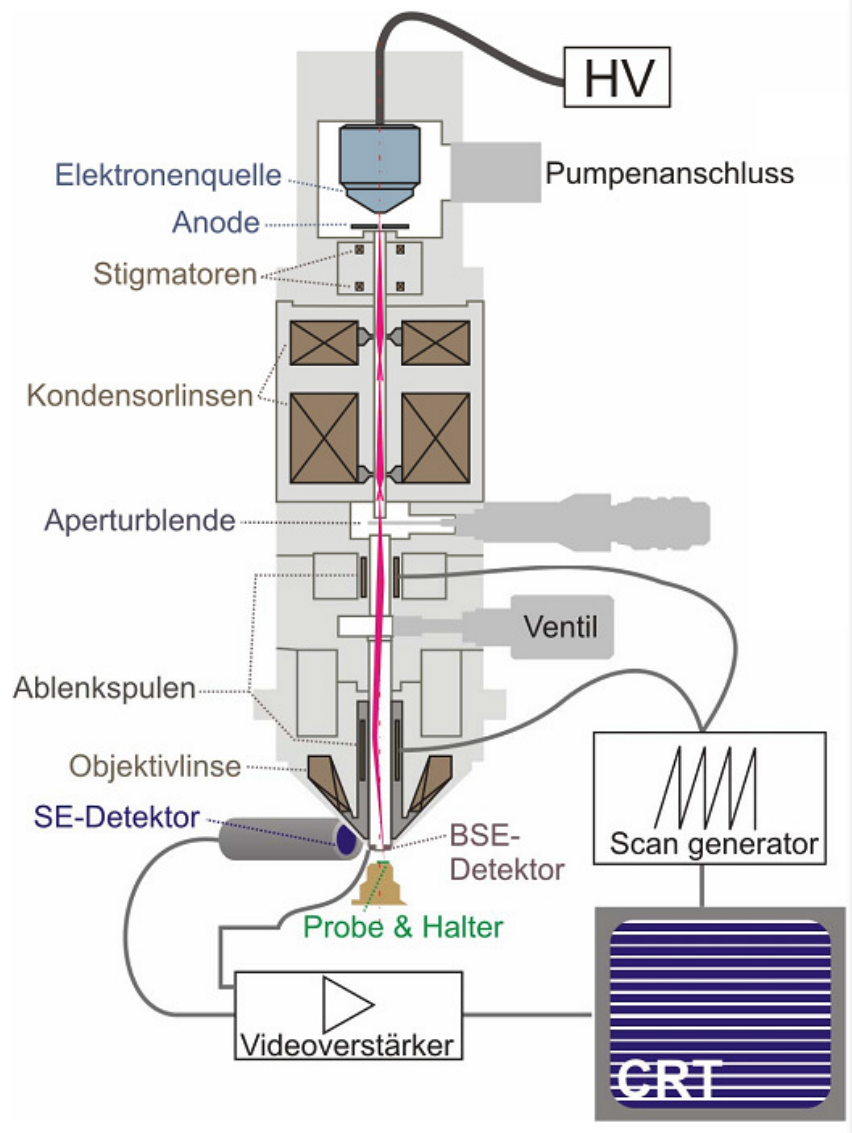
\includegraphics[scale=0.25]{AufbauREM.png}
    \captionof{figure}{Aufbau Raster-Elektronenmikroskop}
    \label{image:aufbau}
\end{center}
\section*{Schärfentiefe}
\begin{center}
    \begin{tabular}{cc}
        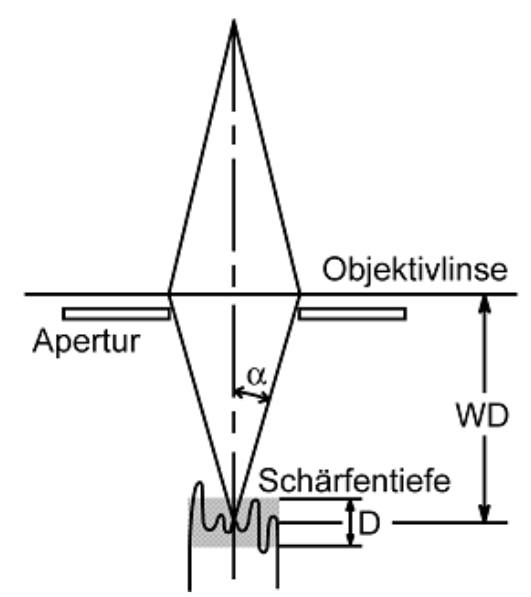
\includegraphics[scale=0.2]{Schaerfentiefe1.png} & 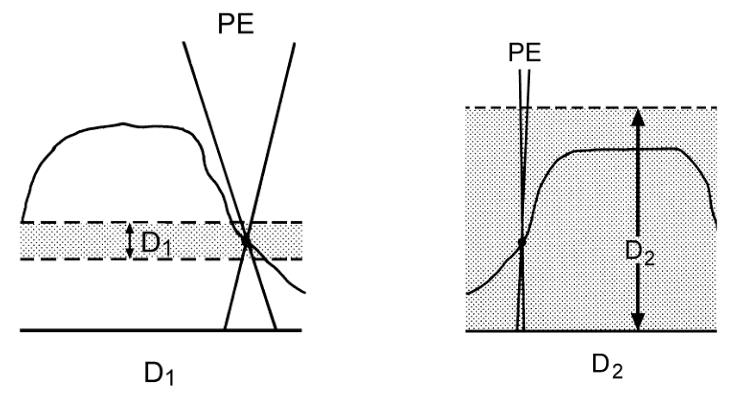
\includegraphics[scale=0.2]{Schaerfentiefe2.png}
    \end{tabular}
    \captionof{figure}{Schärfentiefe}
\end{center}
Die Schärfentiefe eines REM hängt von der Größe der Apertur und dem Arbeitsabstand ab. Dabei gilt kleine Blende und großer Arbeitsabstand besitzt eine hohe Schärfentiefe. Die Schärfentiefe ein Maß, welches angibt in welchen Bereich oberhalb und unterhalb die Probe noch Scharf aufgelöst werden kann.

\section{Wechselwirkung der Elektronen mit Materie}
\label{sec:elektrons}
Durch Wechselwirkung des Primärelektronenstrahls (PE) mit der Materie entstehen unterschiedliche Signale, welche in Abbildung \ref{image:signal} dargestellt sind.
\begin{center}
    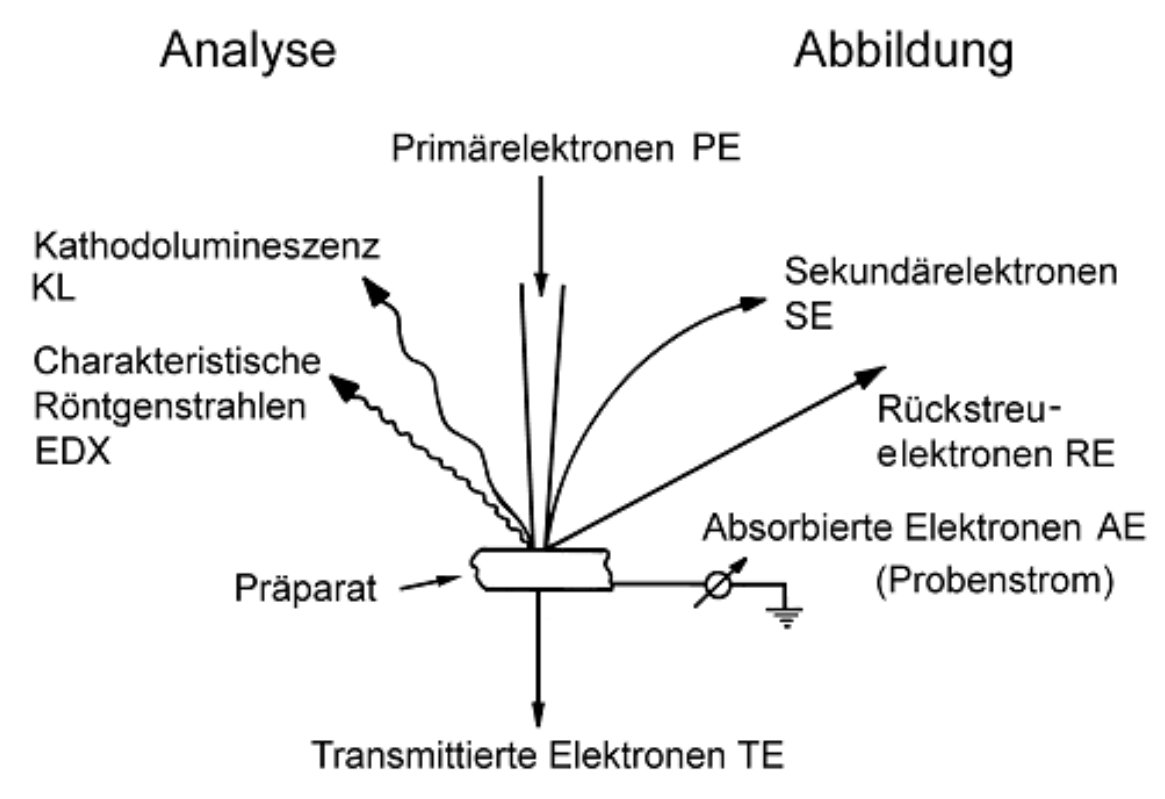
\includegraphics[scale=0.2]{Signalentstehung.png}
    \captionof{figure}{Signale eines REMs}
    \label{image:signal}
\end{center}
Das Volumen, in dem die Elektronen des Primärelektronenstrahls wechselwirken, heißt Streubirne oder Elektronendiffusionswolke, wobei die Reichweite vom gewählten Probenmaterial und der Anregungsspannung abhängt. 
\begin{center}
    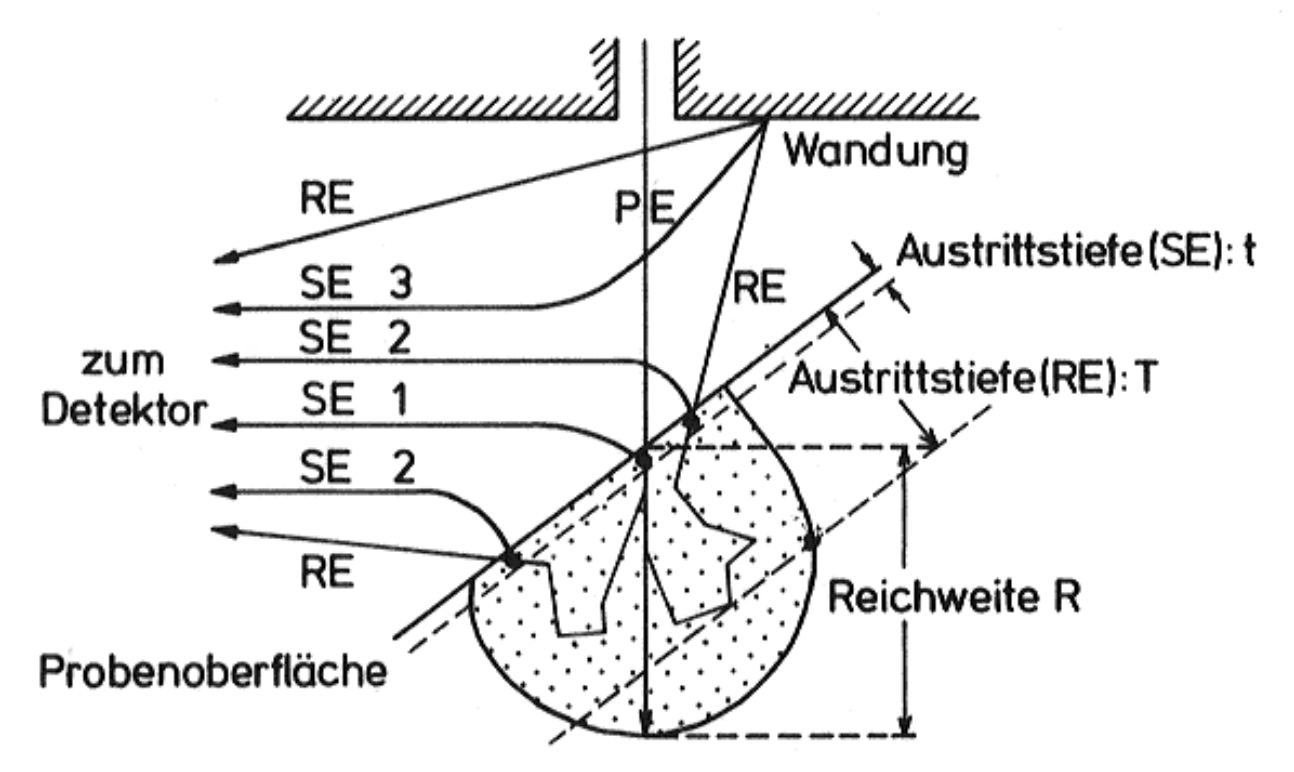
\includegraphics[scale=0.2]{Elektronendiffusionswolke.png}
    \captionof{figure}{Elektronendiffusionswolke}
    \label{image:wolke}
\end{center}
Durch Eindringen des PE entstehen durch unelastische Streuung langsame \textbf{\textit{Sekundärelektronen (SE)}} mit Energie < \SI{50}{\electronvolt} mit wahrscheinlichster Energie $\left\langle E\right\rangle=1-\SI{5}{\electronvolt}$, welche aus der $t =$ 1-\SI{10}{\nano\metre} stammen und zur Hochauflösung des REM führen. \citep{RasterEM} Somit tragen SE maßgeblich zu den dem sogenannten \textit{Topografiekontrast} bei. \citep{WikipolyREM}\\

Elektronen, welche elastisch an Atomkerne gestreut werden und diesen unter großen Winkel verlassen, werden als \textbf{\textit{Rückstoßelektronen (RE)}}. REs haben dabei eine Energie > \SI{50}{\electronvolt}, worunter auch schnellere SE fallen, aber diese sind von REs nicht unterscheidbar sind. Dabei stammen die ausgelösten REs aus einer Materialtiefe $T=$0,1-\SI{1}{\micro\metre} und sind somit verantwortlich für den \textit{Materialkontrast}. Auch hängt die Ausbeute der REs von der Kernladungszahl des Materials ab. \citep{RasterEM} \citep{WikipolyREM} Die REs können auch beim Austreten weitere SEs erzeugen, was man gut Anhand des \textit{Kanteneffekt} erkennen kann. \citep{RasterEM}

\begin{SCfigure}[][h]
    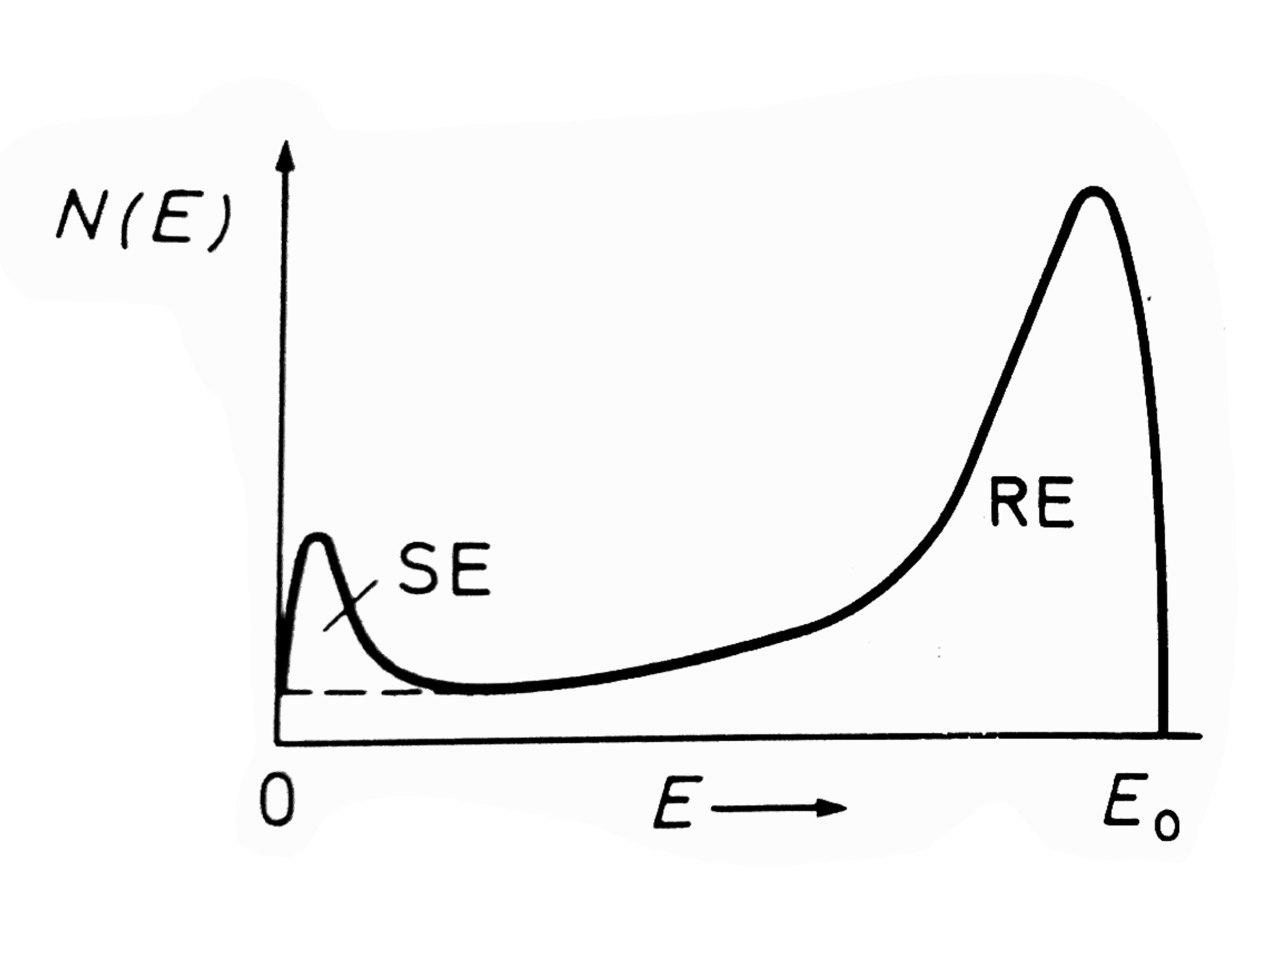
\includegraphics[scale=0.10]{Energieverteilung.jpg}
    \caption{Schematische Energieverteilung der Anzahl von SEs und REs bei normierter Energie}
    \label{image:energieverteilung}
\end{SCfigure}

SEs werden dann in Gruppen unterteilt:
\begin{itemize}
    \item \textbf{SE1:} Aus PE im Material erzeugte SEs
    \item \textbf{SE2:} Aus RE im Material erzeugte SEs 
    \item \textbf{SE3:} Aus RE außerhalb des Materials erzeugte SEs\\   
\end{itemize}

Bis zu einer Reichweite von $R=\SI{500}{\nano\metre}$ entsteht eine Wechselwirkung des PE-Strahls mit der Probe, wobei Elektronen aus der Atomhülle geschlagen werden. Dabei fallen Elektronen aus höheren Zuständen nach und es entsteht dabei Röntgenstrahlung, wobei diese Strahlung charakteristisch für das jeweilige Element ist. Die emittierende Strahlung kann dann noch ein Elektron aus einer höheren Schale herausschlagen, was als Auger-Elektron registriert wird. Bei Kernen mit kleiner Ordnungszahl ($Z$<20) dominiert die Emission von Auger-Elektronen, bei
höheren Ordnungszahlen überwiegt die Emission von charakteristischer Röntgenstrahlung.
\newpage
\section{Detektoren}
\label{sec:detect}

\subsection*{Everheart-Thornley-Detektor}
\label{sub:etDetect}
\begin{center}
    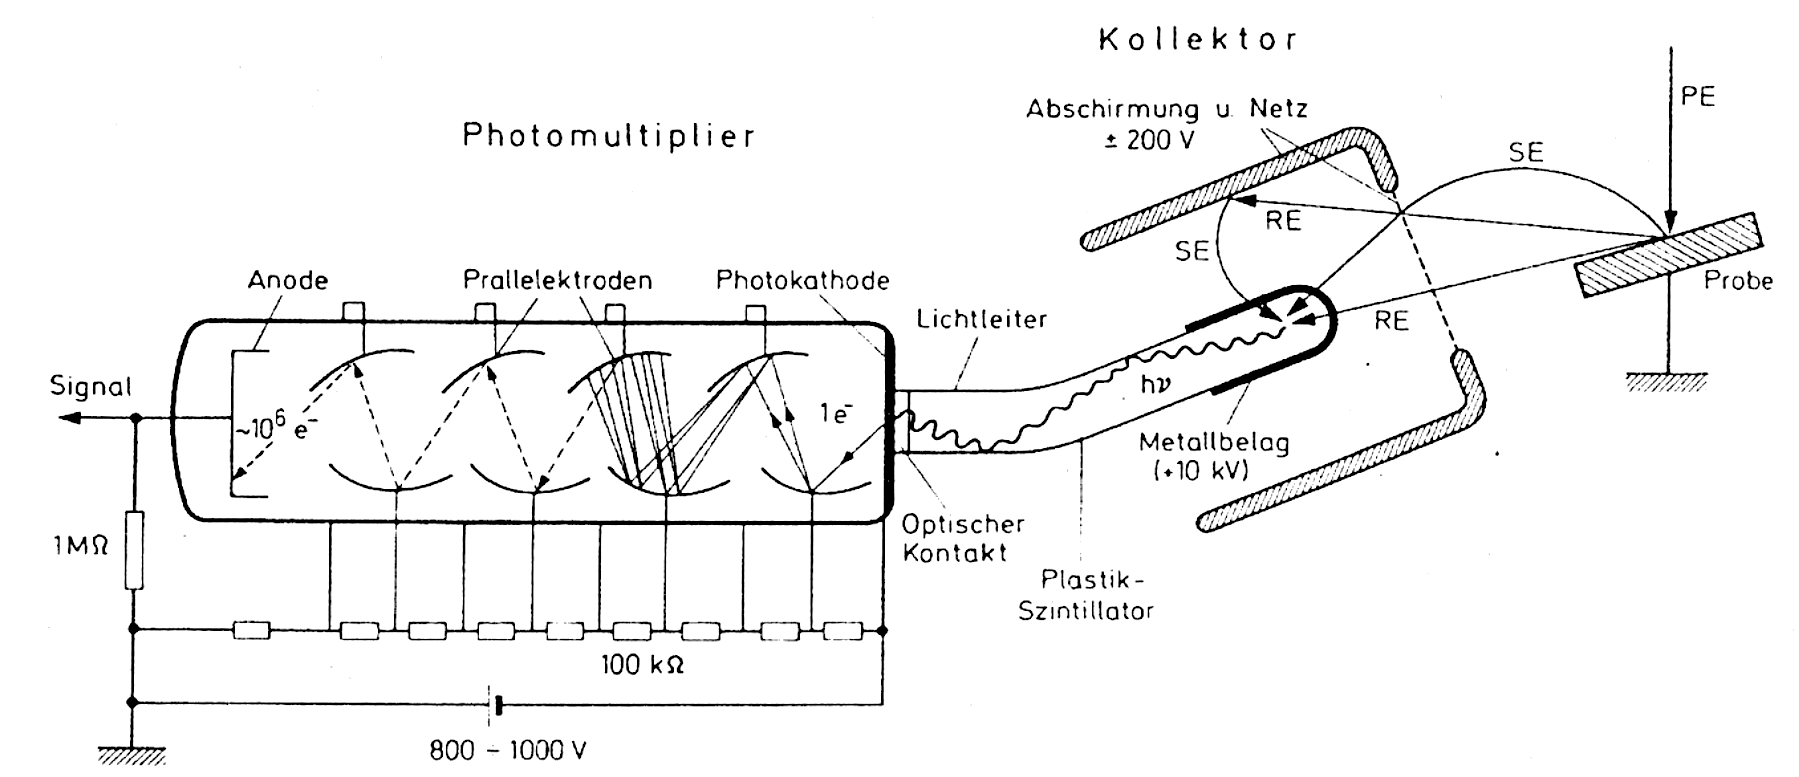
\includegraphics[scale=0.18]{Everheart-Thornley.png}
    \captionof{figure}{Everheart-Thornley-Detektor}
    \label{image:etDetect}
\end{center}
Der Everheart-Thornley-Detektor ist eine Kombination aus Szintillator und Photomultiplier (siehe Abb. \ref{image:etDetect}), welcher zur Detektierung von SEs und REs dient. Die ausgelösten Ses werden dabei von einem Netz des Kollektors mit positiver Spannung angesaugt (mit negativer Spannung können SEs zurückgehalten werden $\Rightarrow$ nur REs im Signal). Schnelle REs, welche einen wesentlich höhere Energie wie SEs haben, passieren das Netz in beiden Fällen. Zwischen Netz und einer \SI{50}{\nano\metre} dünnen leitende Metallschicht auf der Oberfläche des Plastik-Szintillators liegt eine Spannung von \SI{10} {\kilo\volt}, welche die Elektronen zum Szintillator beschleunigen. Dabei entstehen im Szintillator eine große Elektron-Loch-Paar, welcher proportional zur Spannung zwischen Probe und Kollektor und der Neigung der Probe zum Kollektor ist. Die Rekombination dieser Paare erzeugt Lichtquanten, wobei ein großer Teil strahlungslos rekombiniert. Dabei werden die erzeugten Lichtquanten durch Totalreflexion in Richtung des Photomultiplier abgelenkt. Auf der Photokathode wird dann durch das Quant ein Elektron ausgelöst, wobei diese durch eine Prallelektrode auf \SI{100}{\electronvolt} beschleunigt und Spannungsimpulse induzieren, welche wiederum elektronisch verstärkt werden können. Dabei führt jedes einfallende SE mindestens zu einem Spannungsimpuls. Die Spannungsimpuls sorgen dann für einen Steuerung der Bildschirmhelligkeit. \citep{RasterEM}
\newpage
\subsection*{Halbleiterdetektor}
\label{sub:halbDetect}
\begin{center}
    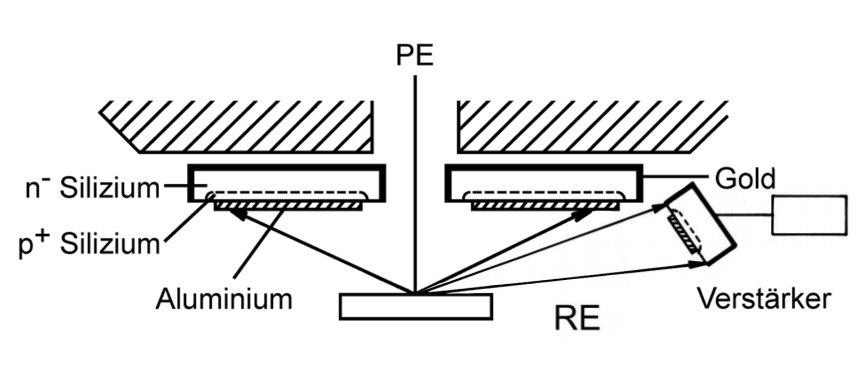
\includegraphics[scale=0.3]{Halbleiterdetektor.jpg}
    \captionof{figure}{Halbleiterdetektor}
    \label{image:halbDetect}
\end{center}
Halbleiterdetektor sind im Grunde Dioden, welche in Sperrrichtung betrieben werden. Dafür eigenen sich diese Detektoren besonders gut für die Untersuchung von REs. Durch das Aluminium wird verhindert, dass Lichtquanten mitdetektiert werden. Auch werden langsame SEs von der Al-Schicht absorbiert. Die REs erzeugen im Leiter Elektron-Loch-Paare, welche dann über den p-n-Übergang diffundieren können, wobei es dort zu Rekombinationen in der jeweiligen Schicht kommt oder getrennt werden. Durch die Trennung der Elektron-Loch-Paare fließt durch den Leiter ein Strom, welcher weiter verstärkt wird und wiederum zur Helligkeitsmodulation dient. Durch seine flache Bauform kann der Halbleiterdetektor nahe an der Probe angebracht werden und füllt zum Gegensatz von (\ref{sub:etDetect}) einen großen Raumwinkel aus. \citep{RasterEM}
\begin{center}
    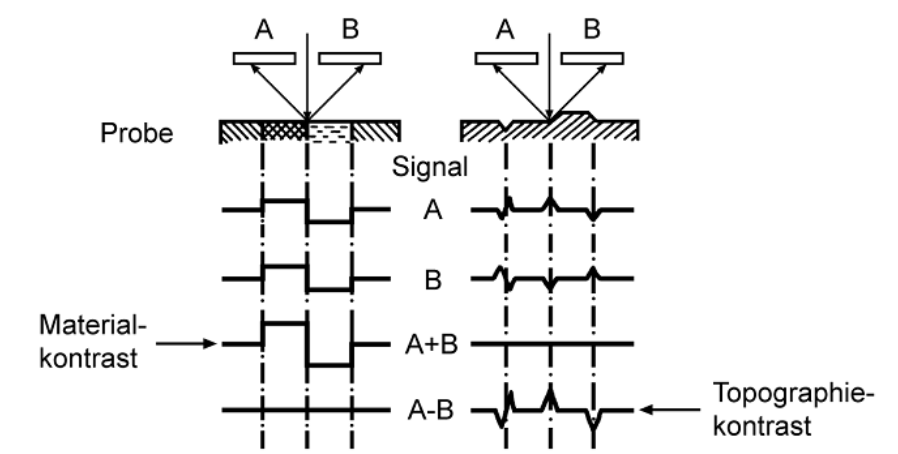
\includegraphics[scale=0.3]{Modi.png}
    \captionof{figure}{Combo- und Topomode}
    \label{image:modi}
\end{center}
Der Halbleiterdetektor kann dabei in verschiedenen Modi betrieben werden (siehe Abb. \ref{image:modi}). Den Combo- (Materialkontrast) und den Topo-Mode (Topografiekontrast).
Weiterhin kann das verwendete Elektronenmikroskop in Praktikum den sogenannten Shadow-Mode, welcher es ermöglicht Combo- und Topo-Mode gleichzeitig zu betrachten. Möglich gemacht wird dies mit Hilfe es dritten Detektor, welcher leicht schräg angewinkelt ist (siehe Abb. \ref{image:halbDetect}).

\subsection*{Si(Li)-Detektor und SDD-Detektor}
\label{sub:siliDetect}
Bei einem Si-Detektor handelt es sich im Grunde um eine in Sperrrichtung betriebenen Silizium-Diode. Dabei Wird bei einer angelegten Sperrspannung eine ladungsträgerfreie Zone(intrinsische Zone) erzeugt. Durch die einfallenden Röntgenquanten werden Elektron-Loch-Paare erzeugt, die durch die angelegte Sperrspannung zu den Elektroden getrennt werden und dabei einen Spannungsimpuls verursachen. Für höhere Effizienz wird die Si-Diode mit Lithium dotiert, womit der Si(Li)-Detektor entsteht. Das Lithium fungiert als Donator und erzeugt mit den p-leitenden Charakter des Siliziums einen p-i-n-Übergang. Um das Driften der Lithium-Ionen zu verhindern, muss der Si(Li)-Detektor permanent gekühlt werden. \citep{RasterEM}
\begin{center}
    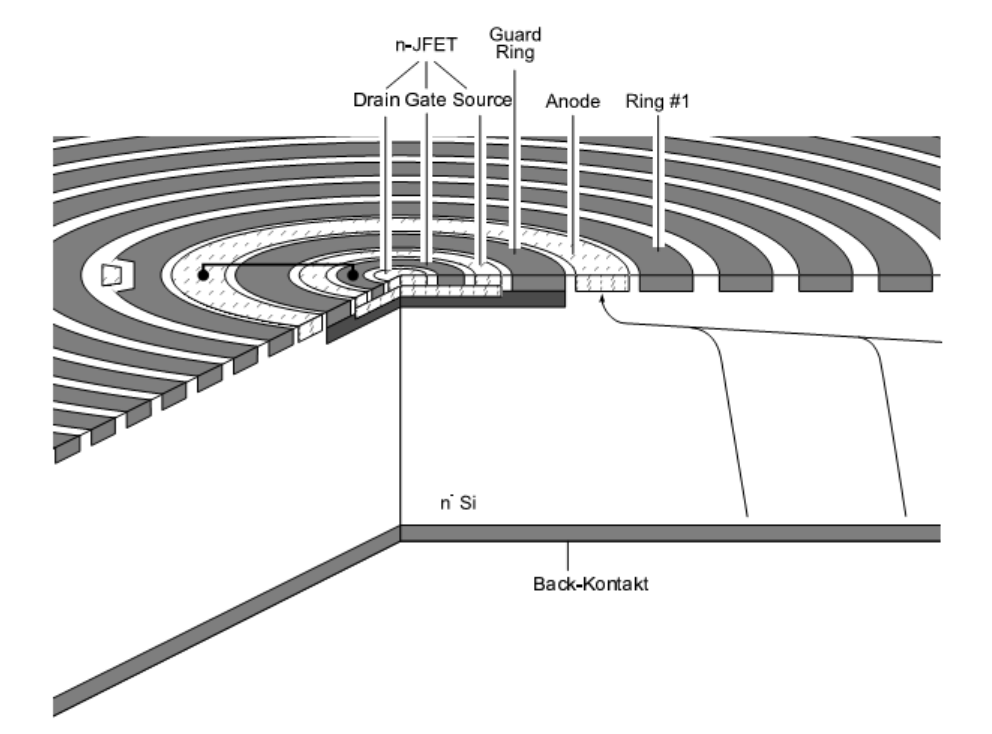
\includegraphics[scale=0.2]{Wafer.png}
    \captionof{figure}{SDD-Detektor}
    \label{image:sddDetect}
\end{center}
Ein Silizium Drift Detektor (SDD) besteht nur aus einem Silizium-Wafer, der mit ringförmigen Elektroden auf der obereren Seite besitzt. Hierbei weist die angelegte Spannung einen Gradienten auf, welcher von Innen nach Außen zunimmt. Als Signalverstärker fungiert ein Feldeffekt Transistor (FET) im Zentrum des Wafers. Der SDD besitzt dabei keine klassische Diodenstruktur und besteht dabei aus zwei gegenüberliegenden p+ dotierten Schichten mit n- dotierter Rückseite als Sammelelektrode. Bei Sperrspannung entsteht auch wieder eine ladungsträgerfreie Zone und ein Potenzialminimum im Zentrum des Wafers, wobei somit ein Spannungsgradient erzeugt wird, der die Elektronen (aus Elektron-Loch-Paar erzeugt durch Röntgenquant) zur Anode leitet und die Löcher zu den Driftringe (siehe Abb. \ref{image:drift}).
\begin{center}
    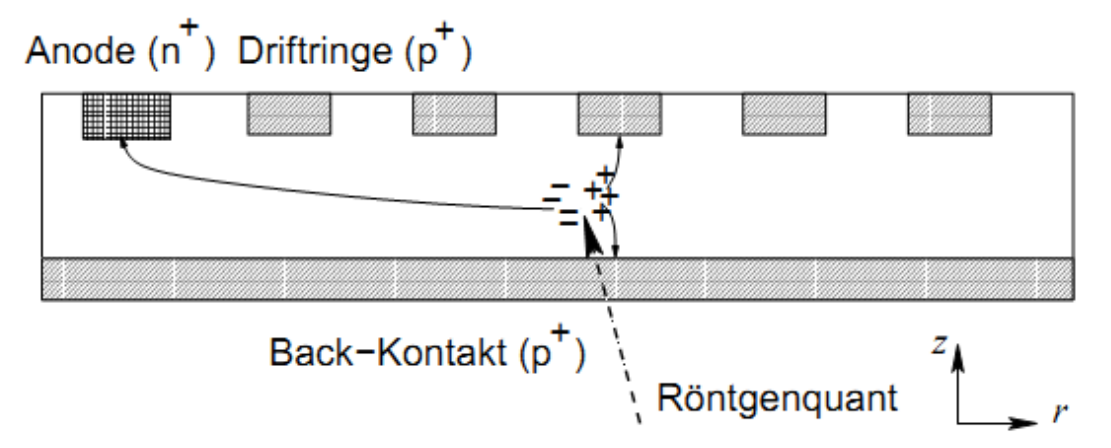
\includegraphics[scale=0.2]{WaferFunk.png}
    \captionof{figure}{Driftfeld SDD-Detektor}
    \label{image:drift}
\end{center}
Der SDD nimmt dabei das klassische Röntgenspektrum (Bremsspektrum, etc.) auf, wobei dabei die $K_\alpha$ für die praktische Analyse am wichtigsten ist, da diese am wahrscheinlichsten entsteht. Die Aufnahme der Spektrallininen kann dabei über wellenlängendispersiv oder energiedispersiv aufgenommen werden. Dabei wird bei einem wellenlängendispersiven Spektrometer (WDS) jeweils auf eine Spektrallinie (mit Hilfe eines Analysatorkristall) direkt eingestellt, wodurch eine genaue Bestimmung der Intensität möglich ist. Bei einem energiedispersiven Spektrometer (EDS) wird simultan das gesamte Röntgenspektrum erfasst wird, was eine gute Übersicht über die auftretenden Linien gibt. Wichtig zu erwähnen ist, dass ein EDS auch bei rauhen Oberflächen ohne Intensitätsabnahme verwendet werden kann, wobei die Messung nur qualitativ ist. Auch ist zu beachten, dass bei einem EDS Überlappungen auftreten können. \citep{RasterEM}
\begin{center}
    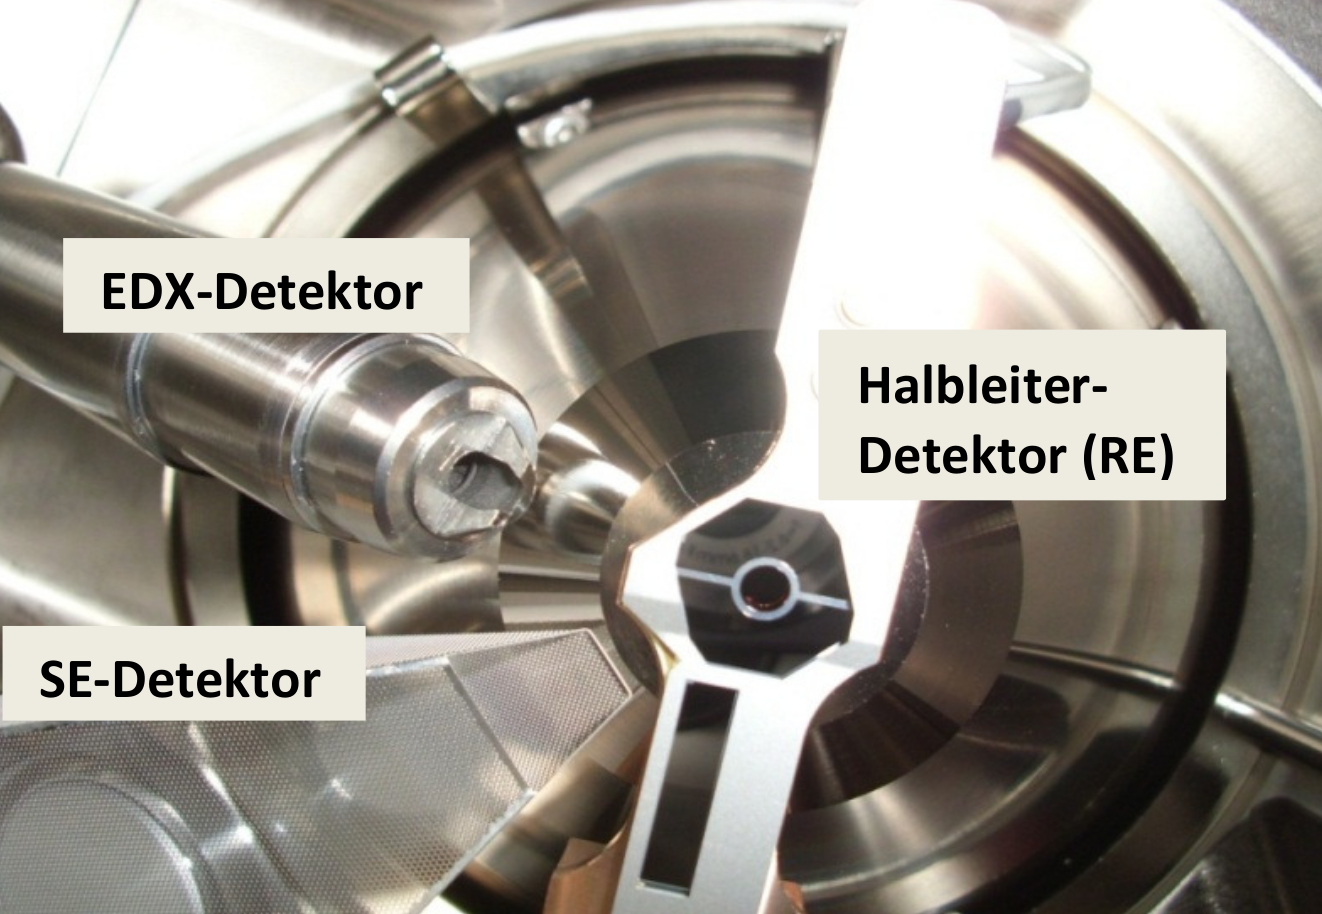
\includegraphics[scale=0.2]{Detektoren.png}
    \captionof{figure}{Detektoren bei Jeol JSM 6510}
    \label{image:jeolDetect}
\end{center}
\newpage
\section{Linsenfehler}
\label{sec:linError}

Bei einem Elektronenmikroskop können auch aufgrund des Welle-Teilchen-Dualismus des Elektrons die bekannten Fehler aus der Optik auftreten. Dabei entstehen folgende Linsenfehler:
\begin{itemize}
    \item[\textbf{1)}]\textbf{Öffnungsfehler:}\\
    Starke Ablenkung und geringere Brennweite bei Strahlen, die in einem großen Abstand von der Achse einfallen. Dabei tretet statt des Brennpunkts ein Kreis mit kleinen Durchmesser auf und der Fehler nimmt mit wachsendem Arbeitsabstand zu (siehe Abb. \ref{image:linError}a). 
    \item[\textbf{2)}]\textbf{Farbfehler (Chromatische Fehler):}\\
    Brennweitendifferenz bei verschiedenen Wellenlängen, wobei dabei ein Zerstreuungskreis entsteht. Durch Stabilisierung der Beschleuigungsspannung und Linsenströme muss dieser Fehler nicht berücksichtigt werden (siehe Abb. \ref{image:linError}b).
    \item[\textbf{3)}]\textbf{Axialer Astigmatismus:}\\
    Durch Fehler in den Elektronenlinsen und der Apperaturblende kann die Brennweite zweier aufeinander senkrecht stehenden ebenen Elektronenbündel eine unterschiedliche Größe haben (siehe Abb. \ref{image:linError}c). Dabei kann der Astigmatismus als Wirkung einer überlagerten Zylinderlinse aufgefasst werden, welcher durch eine zusätzliche senkrechte Zylinderlinse (Stigmator siehe Kapitel \ref{sec:aufbau}) korrigiert werden kann. 
    \item[\textbf{4)}]\textbf{Beugungsfehler:}\\
    Aufgrund Apperaturbegrenzung ist der Fokus nicht scharf, wodurch an einem Punkt neben dem Fokus Interferenzen entstehen und damit ein Beugungsbild (siehe Abb. \ref{image:linError}d).
    \item[\textbf{5)}]\textbf{Zusätzliche Fehler:}\\
    Koma-, Verzeichnung- oder nichtaxiale Farbfehler werden durch kleine Aperturen und Zentrierung des Gerätes korrigiert. \citep{RasterEM}  
\end{itemize}
\newpage
\begin{center}
    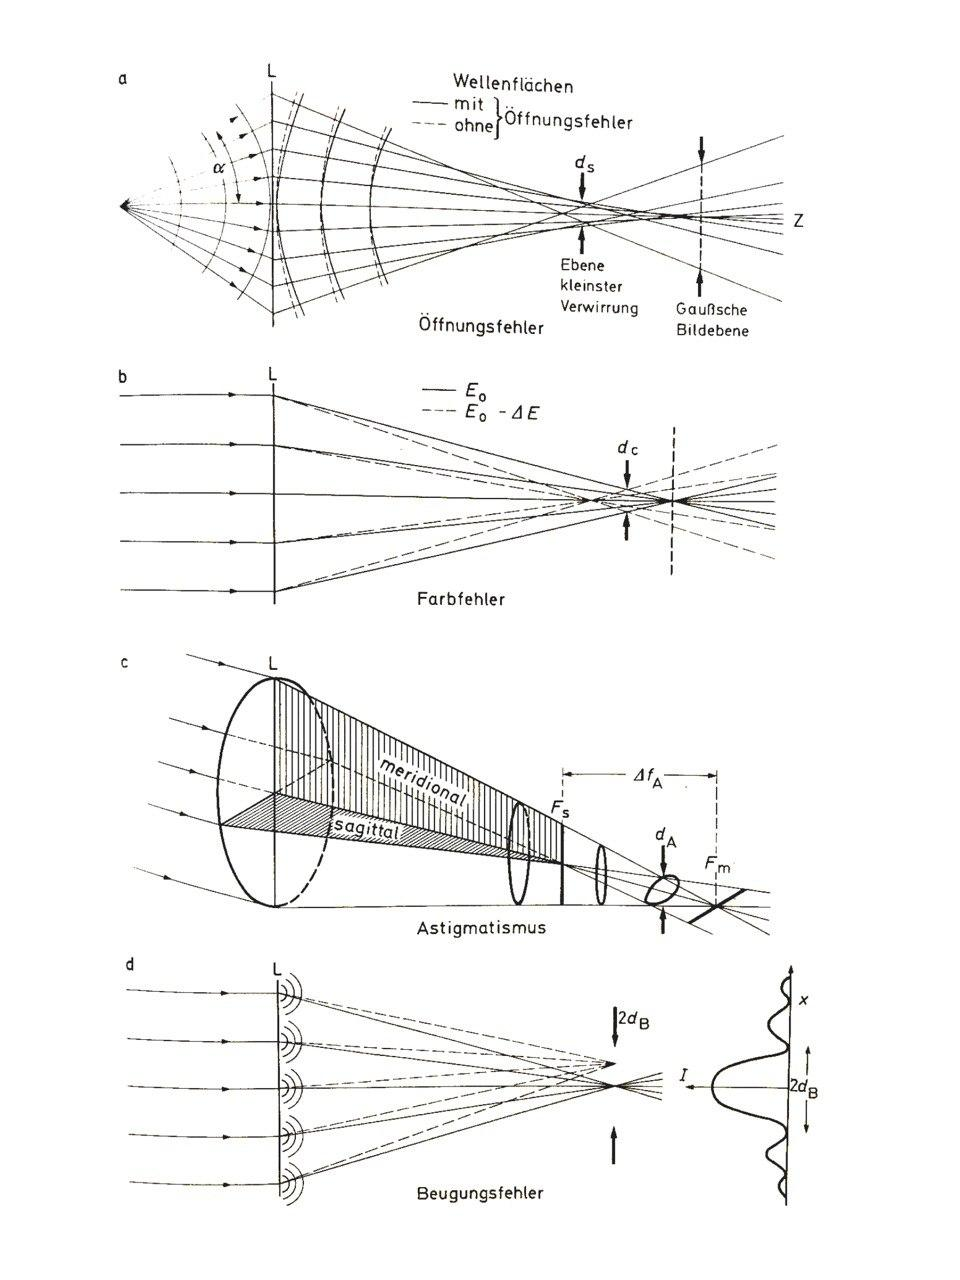
\includegraphics[scale=0.43]{Abbildungsfehler.jpg}
    \captionof{figure}{Linsenfehler}
    \label{image:linError}
\end{center}

\section{Kontraste}
\label{sec:kontrast}

\begin{tabular}{m{0.5\textwidth}m{0.8\textwidth}}
    \textbf{Flächenneigungskontrast} & {}\\
    Der Flächenneigungskontrast durch die Neigung der Probe hin zum Detektor (hier Everhart-Thornley), wodurch die Ausbeute der SE erhöht wird. Durch die Neigung wird die Streubirne (Abb \ref{image:wolke}) abgeschnitten, was zu einer Erhöhung der Fläche, aus welcher die SE treten können, führt. Diese Flächen erscheinen dann im Bild heller als die Flächen vom Detektor weggeneigt. & 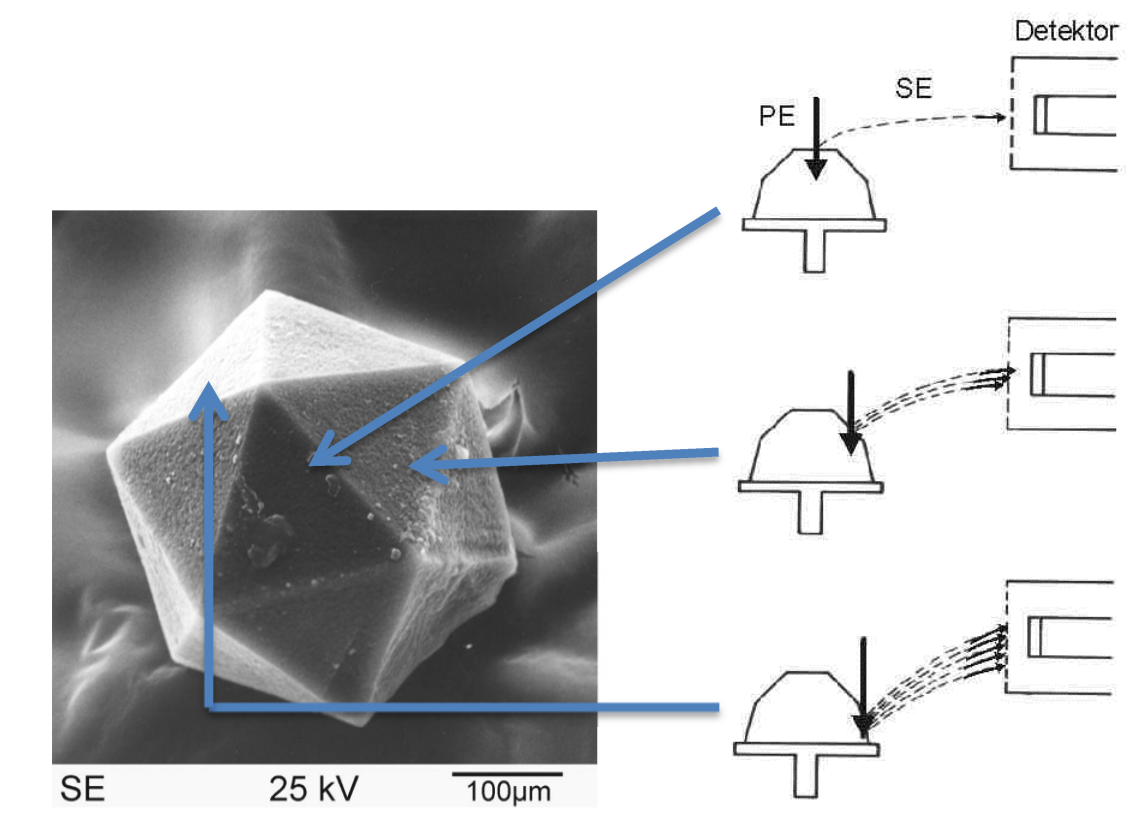
\includegraphics[scale=0.15]{flaechenneigung.png}\\
    {} & {}\\
    \textbf{Kanteneffekt} & {}\\
    Wie in Kapitel \ref{sec:elektrons} erwähnt können RE bei ihrem Austritt aus dem Material SE auslösen. Dies tritt dehr stark an Kanten auf, da dort mehr RE die Probe verlassen können. Dabei bewirkt der Kanteneffekt, dass die genaue Form der Kante sehr schlecht zu erkennen ist. Korrigiert werden kann dies indem die Primärenergie des Elektronenstrahls herabgesetzt wird. & 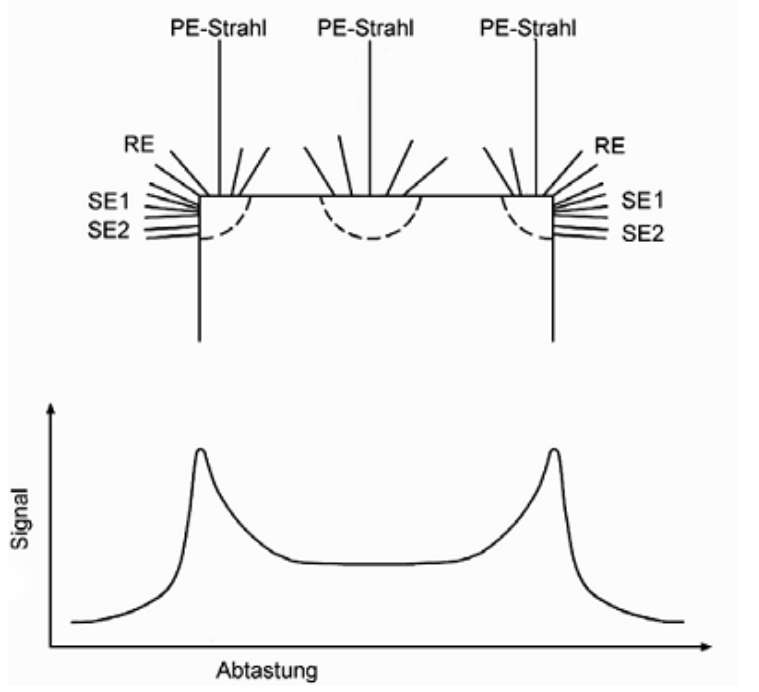
\includegraphics[scale=0.18]{Kanten.png}\\
    {} & {}\\
    \textbf{Abschattungskontrast} & {}\\
    Im Schatten ausgelöste SE können den Kollektor nicht teilweise nicht erreichen, wobei RE auf gradlinigen Bahnen einen sehr scharfen Schatten erzeugen. Schwache Untergrundintensität im Schatten entstehen durch doppelten Rückstreuung der Elektronen an den Probenkammerwänden. & 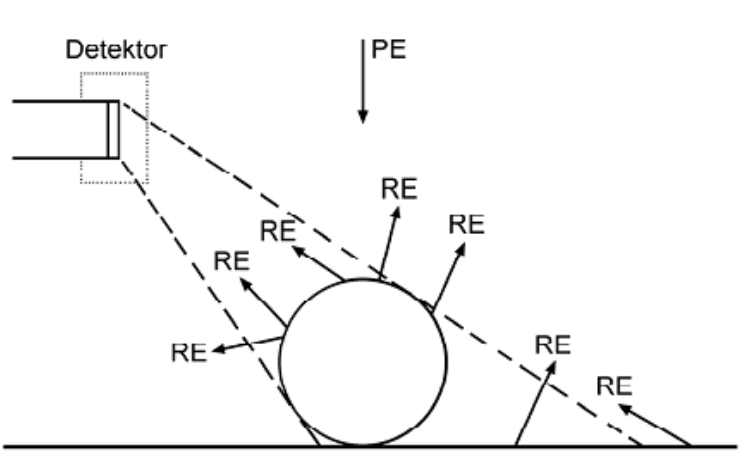
\includegraphics[scale=0.2]{Abschattung.png}\\
    {} & {}\\
    \textbf{Materialkontrast} & {}\\
    Der Materialkontrast entsteht durch eine erhöhte Ausbeute der RE, wodurch Material unterschiedlich hell im Bild erscheinen. Dabei ist die Streuung der RE abhängig von der Kernladungszahl $Z$. Bei höheren $Z$ ist auch der Materialkontrast höher. Wichtig ist dabei, dass die Fläche eben oder der Combomodus (Kapitel \ref{sub:halbDetect}) aktiviert ist. \citep{RasterEM} & 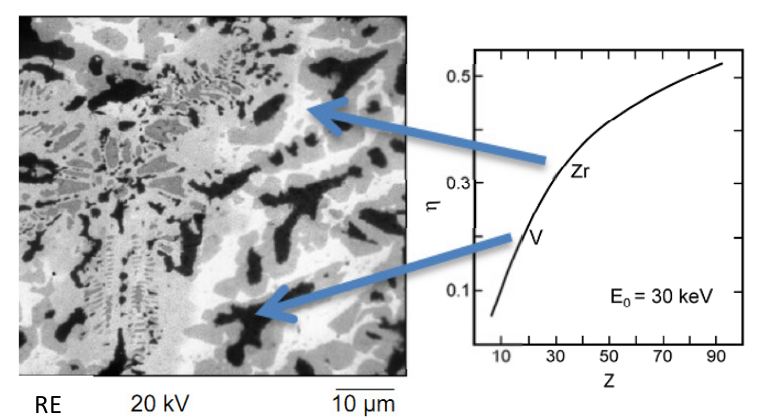
\includegraphics[scale=0.2]{Material.png}
\end{tabular}